% Copyright (C) 2021 Erwin Müller <erwin@muellerpublic.de>
% Released as open-source under the Apache License, Version 2.0.
%
% ****************************************************************************
% ANL-OpenCL :: Docs
% ****************************************************************************
%
% Copyright (C) 2021 Erwin Müller <erwin@muellerpublic.de>
%
% Licensed under the Apache License, Version 2.0 (the "License");
% you may not use this file except in compliance with the License.
% You may obtain a copy of the License at
%
%      http://www.apache.org/licenses/LICENSE-2.0
%
% Unless required by applicable law or agreed to in writing, software
% distributed under the License is distributed on an "AS IS" BASIS,
% WITHOUT WARRANTIES OR CONDITIONS OF ANY KIND, either express or implied.
% See the License for the specific language governing permissions and
% limitations under the License.
%
% ****************************************************************************
% ANL-OpenCL :: Docs is a derivative work based on Josua Tippetts' C++ library:
% http://accidentalnoise.sourceforge.net/index.html
% ****************************************************************************
%
% Copyright (C) 2011 Joshua Tippetts
%
%   This software is provided 'as-is', without any express or implied
%   warranty.  In no event will the authors be held liable for any damages
%   arising from the use of this software.
%
%   Permission is granted to anyone to use this software for any purpose,
%   including commercial applications, and to alter it and redistribute it
%   freely, subject to the following restrictions:
%
%   1. The origin of this software must not be misrepresented; you must not
%      claim that you wrote the original software. If you use this software
%      in a product, an acknowledgment in the product documentation would be
%      appreciated but is not required.
%   2. Altered source versions must be plainly marked as such, and must not be
%      misrepresented as being the original software.
%   3. This notice may not be removed or altered from any source distribution.
%
%
% ****************************************************************************
% ANL-OpenCL :: Docs bundles and uses the RandomCL library:
% https://github.com/bstatcomp/RandomCL
% ****************************************************************************
%
% BSD 3-Clause License
%
% Copyright (c) 2018, Tadej Ciglarič, Erik Štrumbelj, Rok Češnovar. All rights reserved.
%
% Redistribution and use in source and binary forms, with or without modification, are permitted provided that the following conditions are met:
%
% * Redistributions of source code must retain the above copyright notice, this list of conditions and the following disclaimer.
%
% * Redistributions in binary form must reproduce the above copyright notice, this list of conditions and the following disclaimer in the documentation and/or other materials provided with the distribution.
%
% * Neither the name of the copyright holder nor the names of its contributors may be used to endorse or promote products derived from this software without specific prior written permission.
%
% THIS SOFTWARE IS PROVIDED BY THE COPYRIGHT HOLDERS AND CONTRIBUTORS "AS IS" AND ANY EXPRESS OR IMPLIED WARRANTIES, INCLUDING, BUT NOT LIMITED TO, THE IMPLIED WARRANTIES OF MERCHANTABILITY AND FITNESS FOR A PARTICULAR PURPOSE ARE DISCLAIMED. IN NO EVENT SHALL THE COPYRIGHT HOLDER OR CONTRIBUTORS BE LIABLE FOR ANY DIRECT, INDIRECT, INCIDENTAL, SPECIAL, EXEMPLARY, OR CONSEQUENTIAL DAMAGES (INCLUDING, BUT NOT LIMITED TO, PROCUREMENT OF SUBSTITUTE GOODS OR SERVICES; LOSS OF USE, DATA, OR PROFITS; OR BUSINESS INTERRUPTION) HOWEVER CAUSED AND ON ANY THEORY OF LIABILITY, WHETHER IN CONTRACT, STRICT LIABILITY, OR TORT (INCLUDING NEGLIGENCE OR OTHERWISE) ARISING IN ANY WAY OUT OF THE USE OF THIS SOFTWARE, EVEN IF ADVISED OF THE POSSIBILITY OF SUCH DAMAGE.

\subsection{Noise Generation Functions}

Since \ANLOpenCL/ is a port of the Josua Tippetts' C++ library
\url{http://accidentalnoise.sourceforge.net/index.html} the same documentation
can be used for the noise generation functions.
All of the functions and types are defined in the \ANLOpenCLTypeIndex{noise\_gen.h}.

\subsubsection{Value Noise Functions}

\begin{figure}[h]
\centering
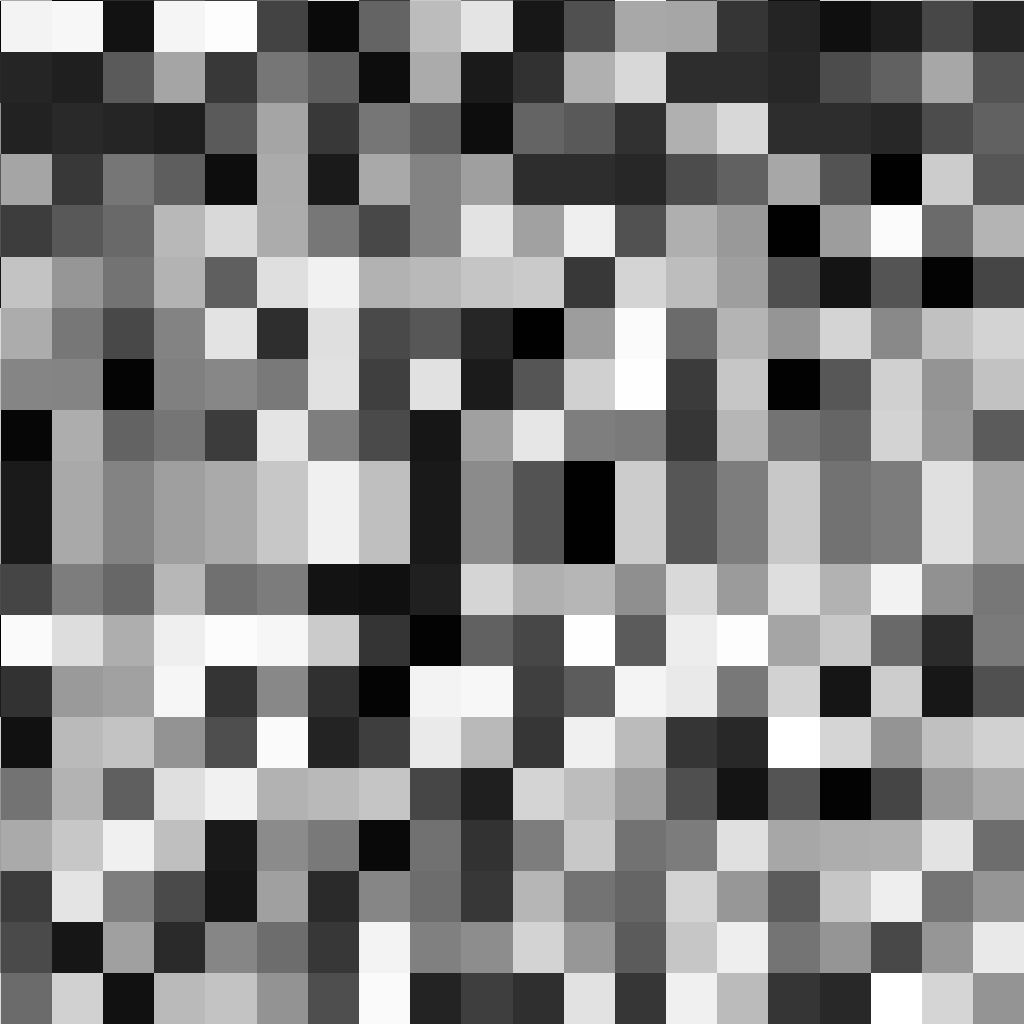
\includegraphics[width=0.4\textwidth]{out/noise_functions/value_noise3D_noInterp.png}
\caption{Value Noise 3D no interpolation.}
\label{fig:value_noise3D_noInterp}
\end{figure}

\begin{figure}[h]
\centering

\includegraphics[width=0.4\textwidth]{out/noise_functions/value_noise3D_linearInterp.png}
\caption{Value Noise 3D linear interpolation.}
\label{fig:value_noise3D_linearInterp}
\end{figure}

\begin{figure}[h]
\centering

\includegraphics[width=0.4\textwidth]{out/noise_functions/value_noise3D_hermiteInterp.png}
\caption{Value Noise 3D hermite interpolation.}
\label{fig:value_noise3D_hermiteInterp}
\end{figure}

\begin{figure}[h]
\centering

\includegraphics[width=0.4\textwidth]{out/noise_functions/value_noise2D_quinticInterp.png}
\caption{Value Noise 3D quintic interpolation.}
\label{fig:value_noise2D_quinticInterp}
\end{figure}

\index{value\_noise2D}\index{value\_noise3D}\index{value\_noise4D}\index{value\_noise6D}
\begin{lstlisting}[caption={Definition of value noise functions},label={lst:value_noise_definition},language=OpenCL]
REAL value_noise2D(vector2 v, uint seed, interp_func interp);
REAL value_noise3D(vector3 v, uint seed, interp_func interp);
REAL value_noise4D(vector4 v, uint seed, interp_func interp);
REAL value_noise6D(vector8 v, uint seed, interp_func interp);
\end{lstlisting}

\begin{lstlisting}[caption={Example for value noise functions},label={lst:value_noise_example},language=OpenCL]
kernel void map2d_image(
global struct SMappingRanges *g_ranges,
write_only image2d_t output
) {
    $insert_localMapRange
    long seed = 200;
    const float v = value_noise3D(coord[i], seed, linearInterp);
    write_imagef(output, (int2)(g0, g1), (float4)(v, v, v, 1.0));
}
\end{lstlisting}

Value noise functions.

\begin{quote}
Value noise is a type of noise commonly used as a procedural texture primitive in computer graphics.
This method consists of the creation of a lattice of points which are assigned random values.
The noise function then returns the interpolated number based on the values of the surrounding lattice points.
\url{https://en.wikipedia.org/wiki/Value_noise}
\end{quote}

\subsubsection{Gradient Noise Functions}

\begin{figure}[h]
\centering
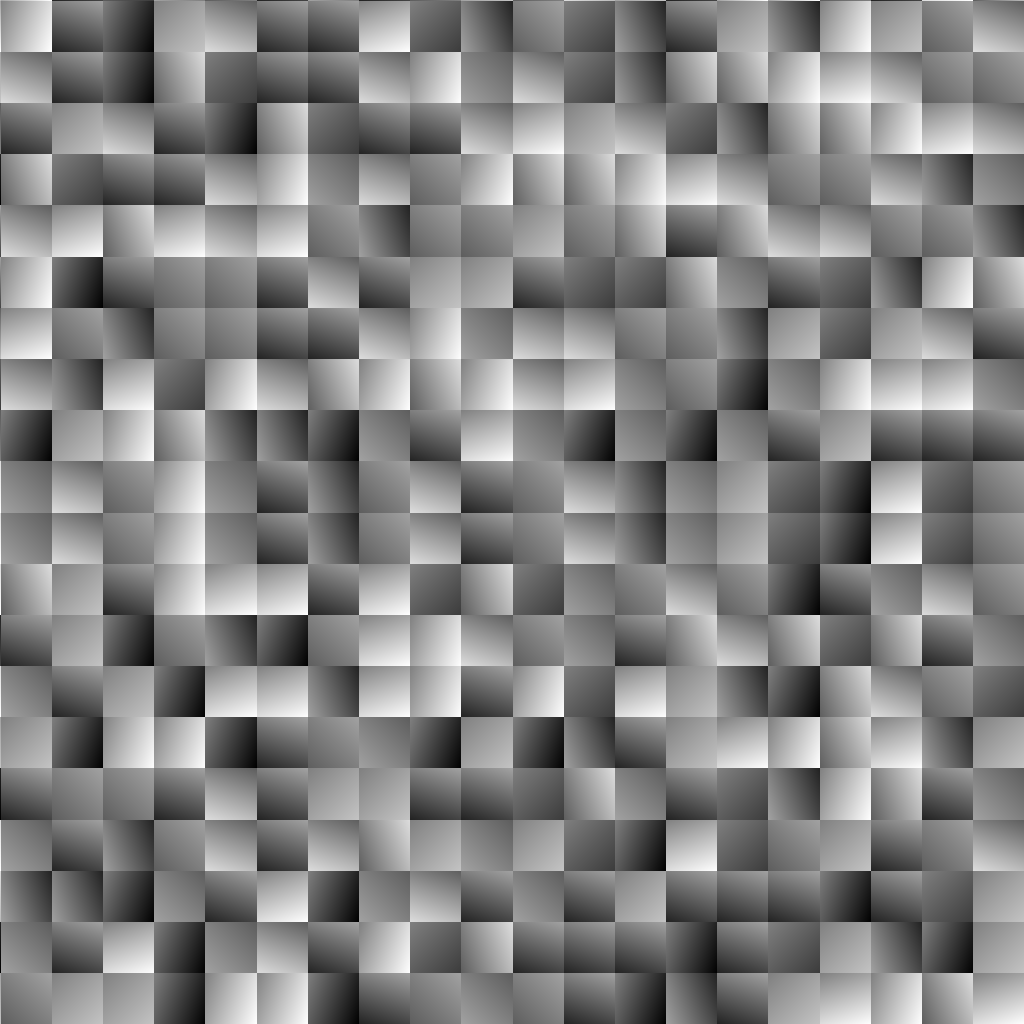
\includegraphics[width=0.4\textwidth]{out/noise_functions/gradient_noise3D_noInterp.png}
\caption{Gradient Noise 3D no interpolation.}
\label{fig:gradient_noise3D_noInterp}
\end{figure}

\begin{figure}[h]
\centering
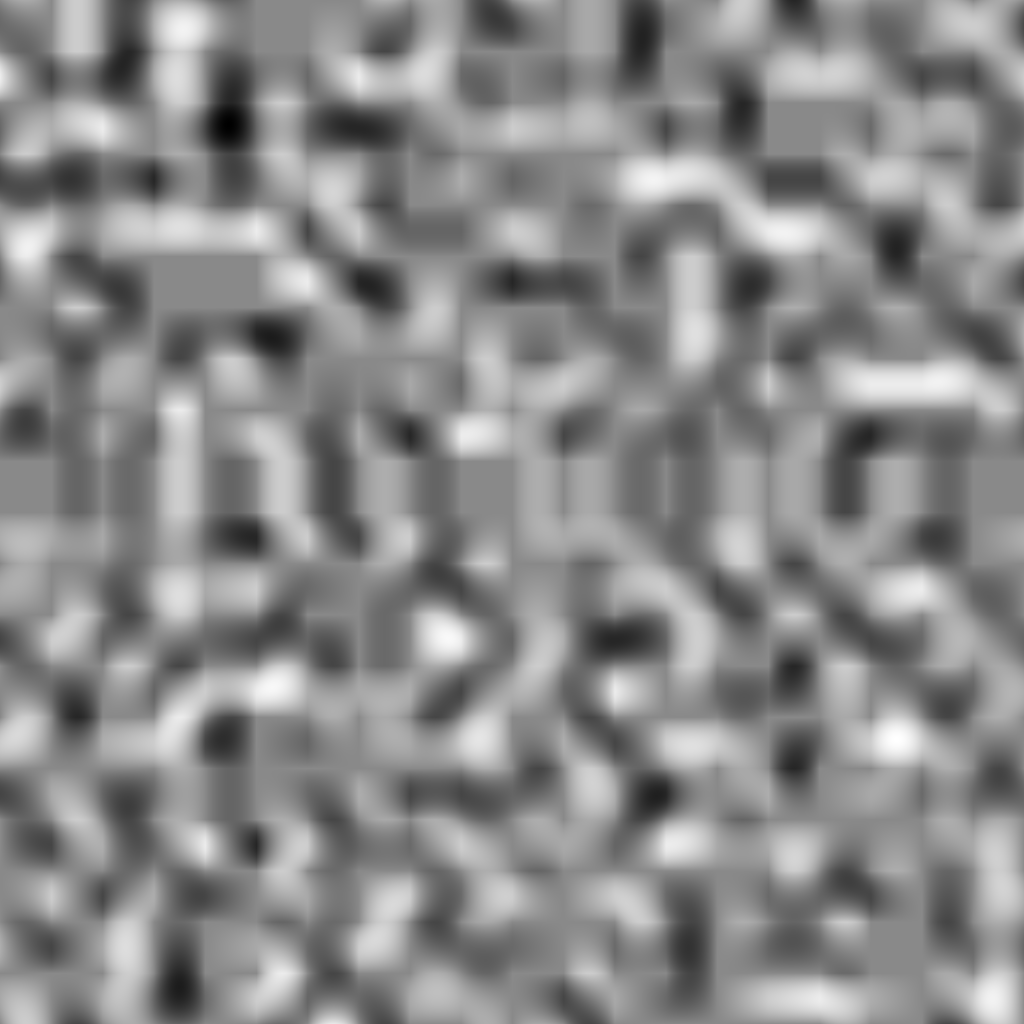
\includegraphics[width=0.4\textwidth]{out/noise_functions/gradient_noise3D_linearInterp.png}
\caption{Gradient Noise 3D linear interpolation.}
\label{fig:gradient_noise3D_linearInterp}
\end{figure}

\begin{figure}[h]
\centering
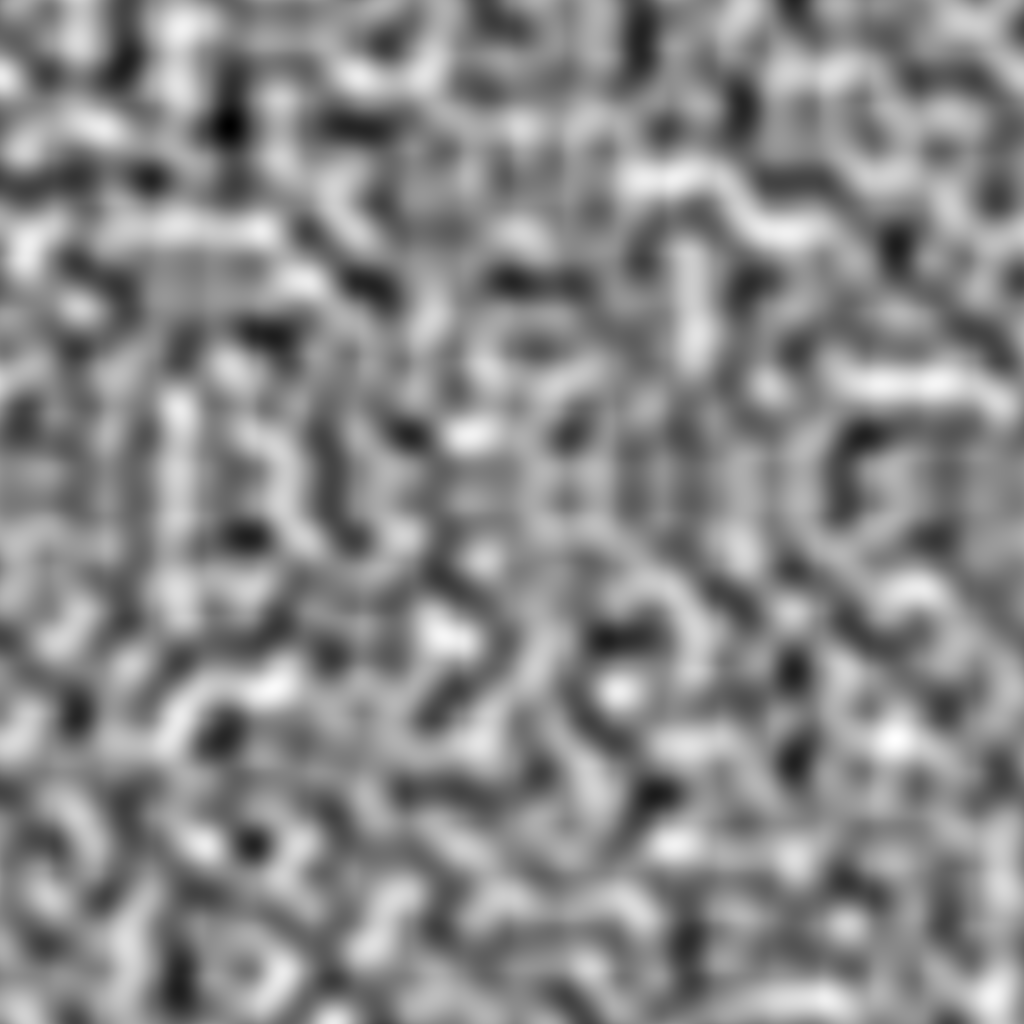
\includegraphics[width=0.4\textwidth]{out/noise_functions/gradient_noise3D_hermiteInterp.png}
\caption{Gradient Noise 3D hermite interpolation.}
\label{fig:gradient_noise3D_hermiteInterp}
\end{figure}

\begin{figure}[h]
\centering
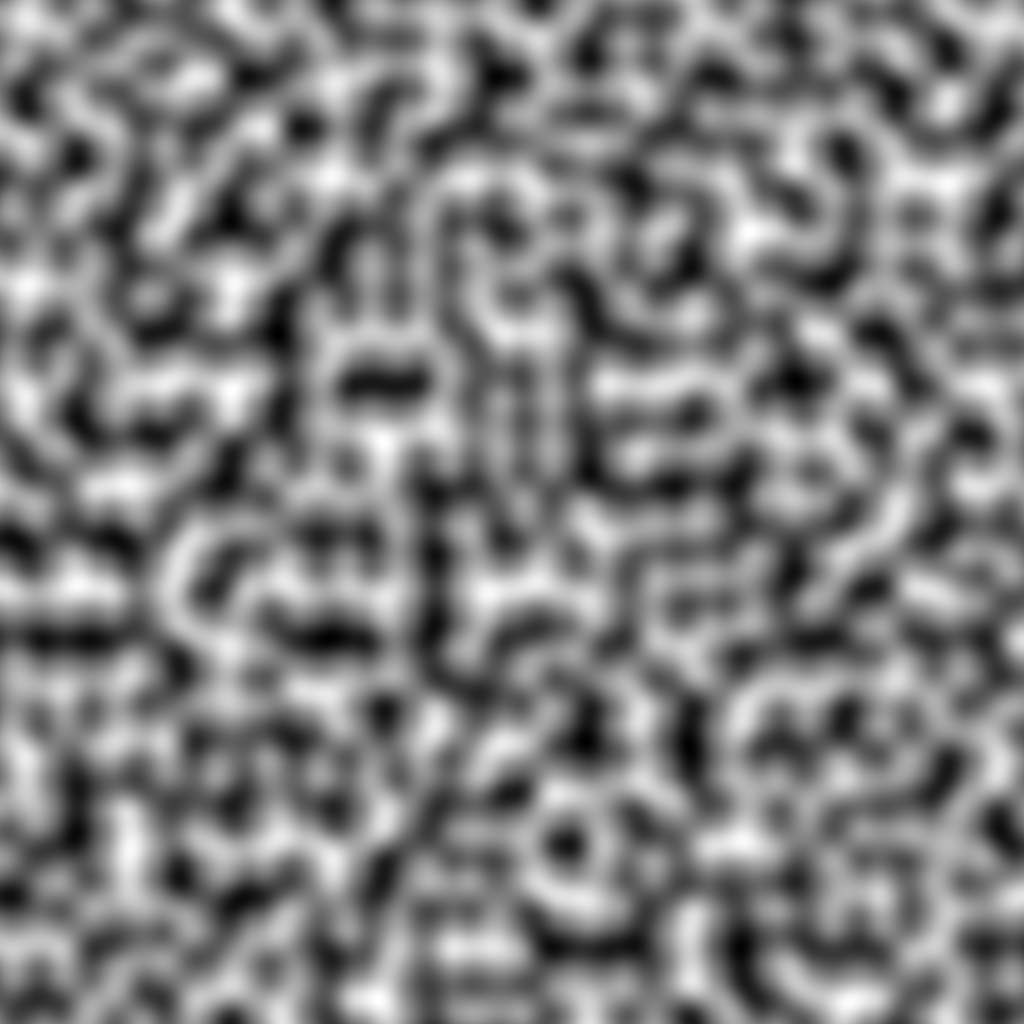
\includegraphics[width=0.4\textwidth]{out/noise_functions/gradient_noise2D_quinticInterp.png}
\caption{Gradient Noise 3D quintic interpolation.}
\label{fig:gradient_noise2D_quinticInterp}
\end{figure}

\index{gradient\_noise2D}\index{gradient\_noise3D}\index{gradient\_noise4D}\index{gradient\_noise6D}
\begin{lstlisting}[caption={Definition of gradient noise functions},label={lst:gradient_noise_definition},language=OpenCL]
REAL gradient_noise2D(vector2 v, uint seed, interp_func interp);
REAL gradient_noise3D(vector3 v, uint seed, interp_func interp);
REAL gradient_noise4D(vector4 v, uint seed, interp_func interp);
REAL gradient_noise6D(vector8 v, uint seed, interp_func interp);
\end{lstlisting}

\begin{lstlisting}[caption={Example for gradient noise functions},label={lst:gradient_noise_example},language=OpenCL]
kernel void map2d_image(
global struct SMappingRanges *g_ranges,
write_only image2d_t output
) {
    $insert_localMapRange
    long seed = 200;
    const float v = gradient_noise3D(coord[i], seed, linearInterp);
    write_imagef(output, (int2)(g0, g1), (float4)(v, v, v, 1.0));
}
\end{lstlisting}

Gradient noise functions.

\begin{quote}
Gradient noise is a type of noise commonly used as a procedural texture primitive in computer graphics.
This method consists of a creation of a lattice of random (or typically pseudorandom) gradients,
dot products of which are then interpolated to obtain values in between the lattices.
An artifact of some implementations of this noise is that the returned value at the lattice points is 0.
Unlike the value noise, gradient noise has more energy in the high frequencies.
\url{https://en.wikipedia.org/wiki/Gradient_noise}
\end{quote}

\subsubsection{Gradval Noise Functions}

\begin{figure}[h]
\centering
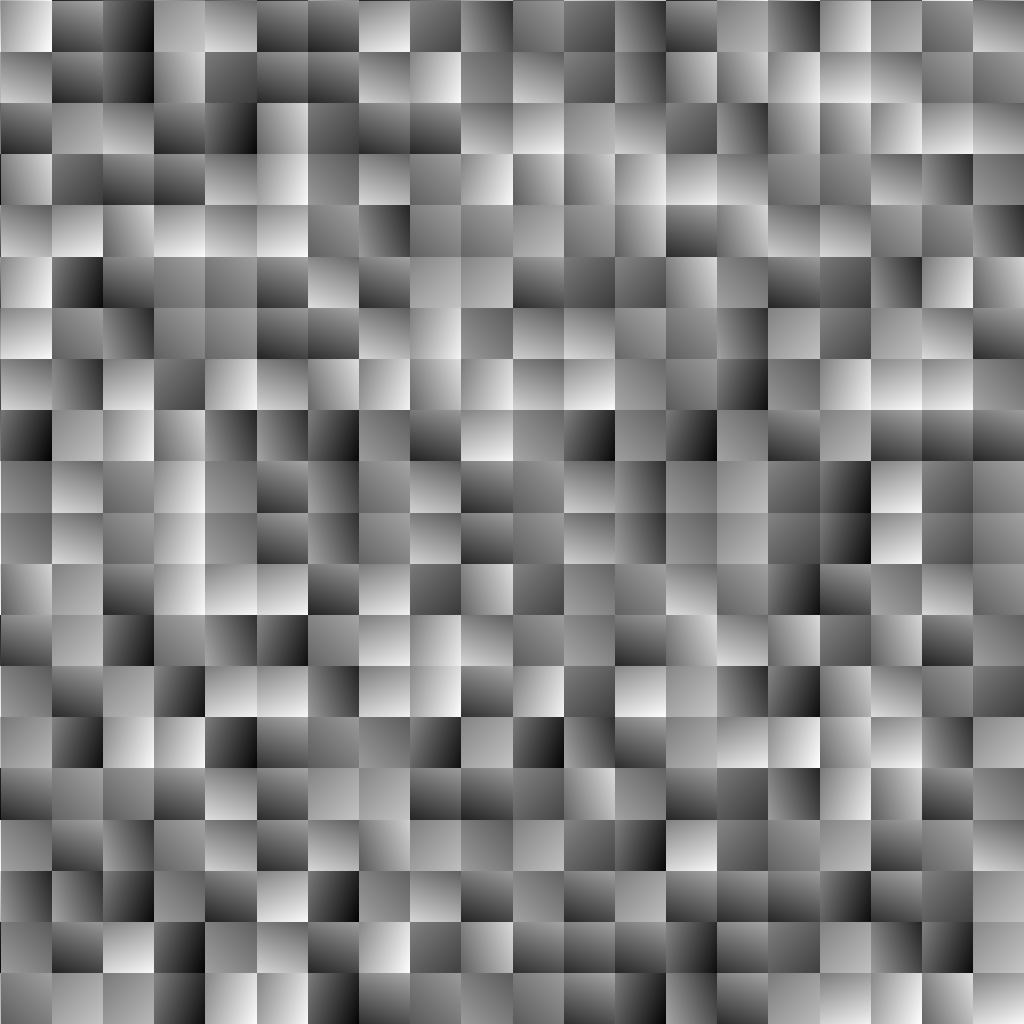
\includegraphics[width=0.4\textwidth]{out/noise_functions/gradval_noise3D_noInterp.png}
\caption{Gradval Noise 3D no interpolation.}
\label{fig:gradval_noise3D_noInterp}
\end{figure}

\begin{figure}[h]
\centering

\includegraphics[width=0.4\textwidth]{out/noise_functions/gradval_noise3D_linearInterp.png}
\caption{Gradval Noise 3D linear interpolation.}
\label{fig:gradval_noise3D_linearInterp}
\end{figure}

\begin{figure}[h]
\centering

\includegraphics[width=0.4\textwidth]{out/noise_functions/gradval_noise3D_hermiteInterp.png}
\caption{Gradval Noise 3D hermite interpolation.}
\label{fig:gradval_noise3D_hermiteInterp}
\end{figure}

\begin{figure}[h]
\centering
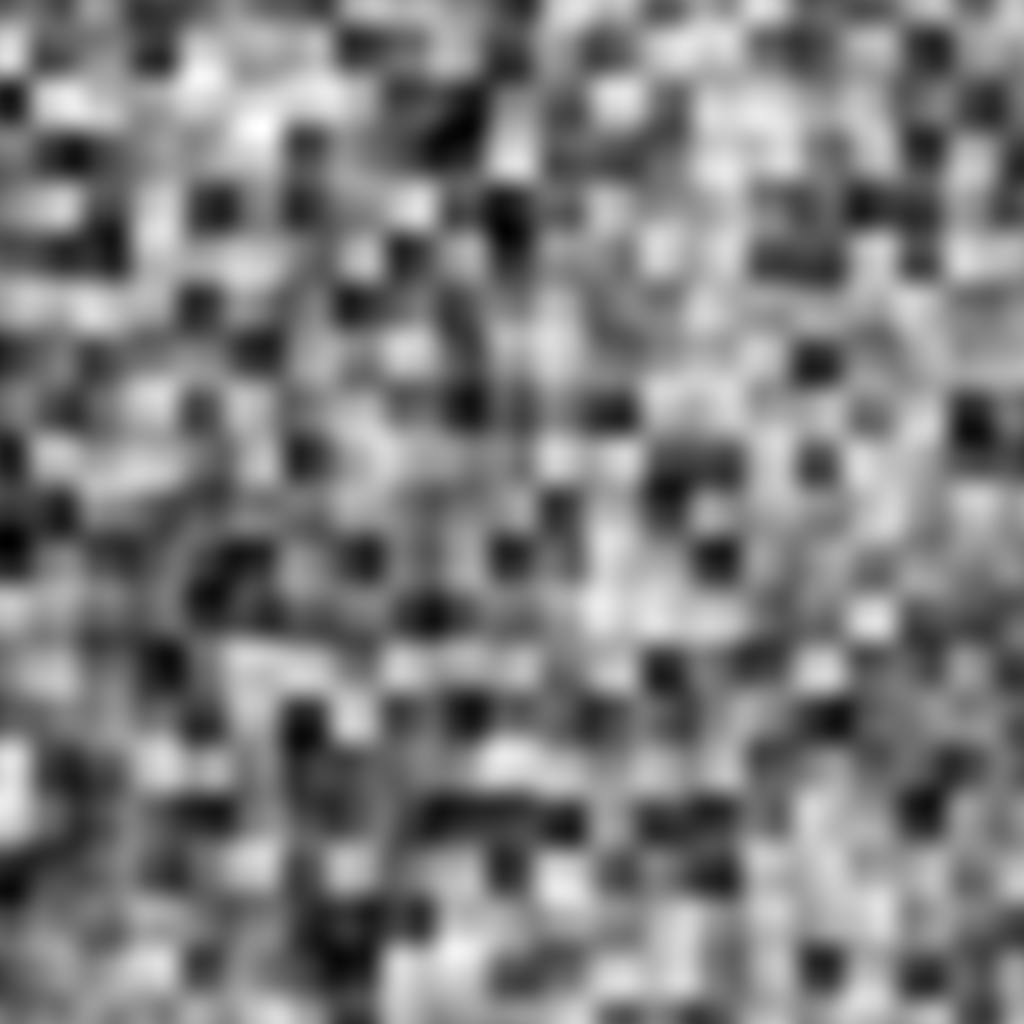
\includegraphics[width=0.4\textwidth]{out/noise_functions/gradval_noise2D_quinticInterp.png}
\caption{Gradval Noise 3D quintic interpolation.}
\label{fig:gradval_noise2D_quinticInterp}
\end{figure}

\index{gradval\_noise2D}\index{gradval\_noise3D}\index{gradval\_noise4D}\index{gradval\_noise6D}
\begin{lstlisting}[caption={Definition of gradval noise functions},label={lst:gradval_noise_definition},language=OpenCL]
REAL gradval_noise2D(vector2 v, uint seed, interp_func interp);
REAL gradval_noise3D(vector3 v, uint seed, interp_func interp);
REAL gradval_noise4D(vector4 v, uint seed, interp_func interp);
REAL gradval_noise6D(vector8 v, uint seed, interp_func interp);
\end{lstlisting}

\begin{lstlisting}[caption={Example for gradval noise functions},label={lst:gradval_noise_example},language=OpenCL]
kernel void map2d_image(
global struct SMappingRanges *g_ranges,
write_only image2d_t output
) {
    $insert_localMapRange
    long seed = 200;
    const float v = gradval_noise3D(coord[i], seed, linearInterp);
    write_imagef(output, (int2)(g0, g1), (float4)(v, v, v, 1.0));
}
\end{lstlisting}

Combined value and gradient noise functions.

\subsubsection{White Noise Functions}

\begin{figure}[h]
\centering
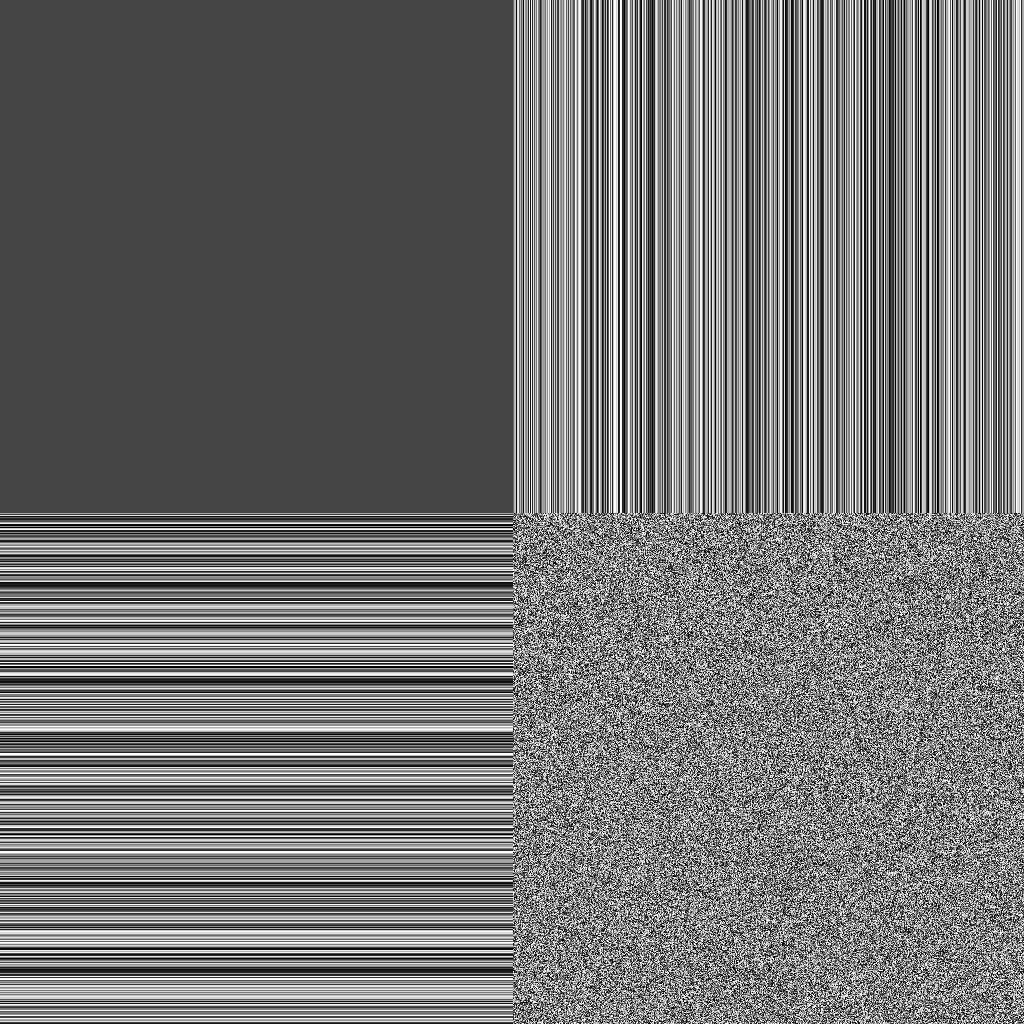
\includegraphics[width=0.4\textwidth]{out/noise_functions/white_noise3D_noInterp.png}
\caption{White Noise 3D no interpolation.}
\label{fig:white_noise3D_noInterp}
\end{figure}

\index{white\_noise2D}\index{white\_noise3D}\index{white\_noise4D}\index{white\_noise6D}
\begin{lstlisting}[caption={Definition of white noise functions},label={lst:white_noise_definition},language=OpenCL]
REAL white_noise2D(vector2 v, uint seed, interp_func interp);
REAL white_noise3D(vector3 v, uint seed, interp_func interp);
REAL white_noise4D(vector4 v, uint seed, interp_func interp);
REAL white_noise6D(vector8 v, uint seed, interp_func interp);
\end{lstlisting}

\begin{lstlisting}[caption={Example for white noise functions},label={lst:white_noise_example},language=OpenCL]
kernel void map2d_image(
global struct SMappingRanges *g_ranges,
write_only image2d_t output
) {
    $insert_localMapRange
    long seed = 200;
    const float v = white_noise3D(coord[i], seed, linearInterp);
    write_imagef(output, (int2)(g0, g1), (float4)(v, v, v, 1.0));
}
\end{lstlisting}

White noise functions. The interpolation function parameter is not used.
The interpolation function parameter is only for compatibility with
the other noise functions.

\begin{quote}
In signal processing, white noise is a random signal having equal
intensity at different frequencies, giving it a constant power spectral density.
\url{https://en.wikipedia.org/wiki/White_noise}
\end{quote}

\subsubsection{Simplex Noise Functions}

\begin{figure}[h]
\centering

\includegraphics[width=0.4\textwidth]{out/noise_functions/simplex_noise3D_noInterp.png}
\caption{Simplex Noise 3D no interpolation.}
\label{fig:simplex_noise3D_noInterp}
\end{figure}

\index{simplex\_noise2D}\index{simplex\_noise3D}\index{simplex\_noise4D}\index{simplex\_noise6D}
\begin{lstlisting}[caption={Definition of simplex noise functions},label={lst:simplex_noise_definition},language=OpenCL]
REAL simplex_noise2D(vector2 v, uint seed, interp_func interp);
REAL simplex_noise3D(vector3 v, uint seed, interp_func interp);
REAL simplex_noise4D(vector4 v, uint seed, interp_func interp);
REAL simplex_noise6D(vector8 v, uint seed, interp_func interp);
\end{lstlisting}

\begin{lstlisting}[caption={Example for simplex noise functions},label={lst:simplex_noise_example},language=OpenCL]
kernel void map2d_image(
global struct SMappingRanges *g_ranges,
write_only image2d_t output
) {
    $insert_localMapRange
    long seed = 200;
    const float v = simplex_noise3D(coord[i], seed, linearInterp);
    write_imagef(output, (int2)(g0, g1), (float4)(v, v, v, 1.0));
}
\end{lstlisting}

Simplex noise functions. The interpolation function parameter is not used.
The interpolation function parameter is only for compatibility with
the other noise functions.

\begin{quote}
Simplex noise is a method for constructing an n-dimensional noise function
comparable to Perlin noise ("classic" noise) but with fewer directional
artifacts and, in higher dimensions, a lower computational overhead.
\url{https://en.wikipedia.org/wiki/Simplex_noise}
\end{quote}

\subsubsection{Cellular Noise Functions}

\index{cellular\_function2D}\index{cellular\_function3D}\index{cellular\_function4D}\index{cellular\_function6D}
\begin{lstlisting}[caption={Definition of cellular noise functions},label={lst:cellular_noise_definition},language=OpenCL]
REAL cellular_function2D(vector2 v, uint seed, REAL *f, REAL *disp, dist_func2 distance);
REAL cellular_function3D(vector3 v, uint seed, REAL *f, REAL *disp, dist_func3 distance);
REAL cellular_function4D(vector4 v, uint seed, REAL *f, REAL *disp, dist_func4 distance);
REAL cellular_function6D(vector8 v, uint seed, REAL *f, REAL *disp, dist_func6 distance);
\end{lstlisting}

\begin{lstlisting}[caption={Example for cellular noise functions},label={lst:cellular_noise_example},language=OpenCL]
kernel void map2d_image(
global struct SMappingRanges *g_ranges,
write_only image2d_t output
) {
    $insert_localMapRange
    long seed = 200;
    REAL f[4] = { 10, 5, 2.5, 1.25 };
    REAL disp[4] = { 100, 50, 25, 10 };
    const float v = cellular_function3D(coord[i], seed, f, disp, distEuclid3);
    write_imagef(output, (int2)(g0, g1), (float4)(v, v, v, 1.0));
}
\end{lstlisting}

Cellular noise functions. 
Compute distance (for cellular modules) and displacement (for voronoi modules).

\subsubsection{Interpolation Functions}

\index{noInterp}\index{linearInterp}\index{hermiteInterp}\index{quinticInterp}
\begin{lstlisting}[caption={Definition of interpolation functions},label={lst:interpolation_definition},language=OpenCL]
REAL noInterp(REAL t);
REAL linearInterp(REAL t);
REAL hermiteInterp(REAL t);
REAL quinticInterp(REAL t);
\end{lstlisting}

\begin{lstlisting}[caption={Example for interpolation functions},label={lst:interpolation_example},language=OpenCL]
const float v = cellular_noise3D(coord[i], seed, noInterp);
// or
const float v = cellular_noise3D(coord[i], seed, linearInterp);
// or
const float v = cellular_noise3D(coord[i], seed, hermiteInterp);
// or
const float v = cellular_noise3D(coord[i], seed, quinticInterp);
\end{lstlisting}

The four interpolation functions are provided for the noise generation functions.
The functions are not used directly but specified as a parameter.

\index{interp\_func}
\begin{lstlisting}[caption={Definition of interpolation function type},label={lst:interpolation_definition_type},language=OpenCL]
typedef REAL (*interp_func)(REAL);
\end{lstlisting}

The interpolation functions take an input of the type \ANLOpenCLType{REAL} that
is either type \code{float} or \code{double} and returns the interpolated value
that is also of type \ANLOpenCLType{REAL}.

\subsubsection{Noise Generation Function Types}

\index{noise\_func2}\index{noise\_func3}\index{noise\_func4}\index{noise\_func6}
\begin{lstlisting}[caption={Definition of noise generation function types},label={lst:noise_functions_types},language=OpenCL]
typedef REAL (*noise_func2)(vector2, uint, interp_func);
typedef REAL (*noise_func3)(vector3, uint, interp_func);
typedef REAL (*noise_func4)(vector4, uint, interp_func);
typedef REAL (*noise_func6)(vector8, uint, interp_func);
\end{lstlisting}

The noise generation functions can be used as parameters to other generation
functions. Those are the definitions for 2D, 3D, 4D and 6D noise functions types.
The parameters are described below.

\begin{enumerate}
\item expects the 2D, 3D, 4D or 6D coordinate;
\item expects the seed;
\item expects interpolation function;
\end{enumerate}

\subsubsection{Distance Functions}

\index{distEuclid2}\index{distEuclid3}\index{distEuclid4}\index{distEuclid6}
\begin{lstlisting}[caption={Definition of Euclid distance functions},label={lst:distance_euclid_functions},language=OpenCL]
REAL distEuclid2(vector2 a, vector2 b);
REAL distEuclid3(vector3 a, vector3 b);
REAL distEuclid4(vector4 a, vector4 b);
REAL distEuclid6(vector8 a, vector8 b);
\end{lstlisting}

Returns the Euclidean distance between two points $a$ and $b$ as $d(a,b) = |a-b|$.

\index{distManhattan2}\index{distManhattan3}\index{distManhattan4}\index{distManhattan6}
\begin{lstlisting}[caption={Definition of Manhattan distance functions},label={lst:distance_manhattan_functions},language=OpenCL]
REAL distManhattan2(vector2 a, vector2 b);
REAL distManhattan3(vector3 a, vector3 b);
REAL distManhattan4(vector4 a, vector4 b);
REAL distManhattan6(vector8 a, vector8 b);
\end{lstlisting}

Returns the Manhattan distance between two points.

\begin{quote}
A taxicab geometry is a form of geometry in which the usual distance function or metric of Euclidean geometry is replaced by a new metric in which the distance between two points is the sum of the absolute differences of their Cartesian coordinates.
\url{https://en.wikipedia.org/wiki/Taxicab_geometry}
\end{quote}

\index{distGreatestAxis2}\index{distGreatestAxis3}\index{distGreatestAxis4}\index{distGreatestAxis6}
\begin{lstlisting}[caption={Definition of greatest axis distance functions},label={lst:distance_greatest_axis_functions},language=OpenCL]
REAL distGreatestAxis2(vector2 a, vector2 b);
REAL distGreatestAxis3(vector3 a, vector3 b);
REAL distGreatestAxis4(vector4 a, vector4 b);
REAL distGreatestAxis6(vector8 a, vector8 b);
\end{lstlisting}

Returns the distance between two points on the axis that have the greatest distance.

\index{distLeastAxis2}\index{distLeastAxis3}\index{distLeastAxis4}\index{distLeastAxis6}
\begin{lstlisting}[caption={Definition of least axis distance functions},label={lst:distance_least_axis_functions},language=OpenCL]
REAL distLeastAxis2(vector2 a, vector2 b);
REAL distLeastAxis3(vector3 a, vector3 b);
REAL distLeastAxis4(vector4 a, vector4 b);
REAL distLeastAxis6(vector8 a, vector8 b);
\end{lstlisting}

Returns the distance between two points on the axis that have the least distance.

\subsubsection{Distance Function Types}

\index{dist\_func2}\index{dist\_func3}\index{dist\_func4}\index{dist\_func6}
\begin{lstlisting}[caption={Definition of distance function types},label={lst:distance_functions_types},language=OpenCL]
typedef REAL (*dist_func2)(vector2, vector2);
typedef REAL (*dist_func3)(vector3, vector3);
typedef REAL (*dist_func4)(vector4, vector4);
typedef REAL (*dist_func6)(vector8, vector8);
\end{lstlisting}

The distance functions can be used as parameters to other generation
functions. Those are the definitions for 2D, 3D, 4D and 6D noise functions types.
The parameters are described below. Returns the distance between the two coordinates.

\begin{enumerate}
\item expects the first 2D, 3D, 4D or 6D coordinate;
\item expects the second 2D, 3D, 4D or 6D coordinate;
\end{enumerate}
